\documentclass[10pt,a4paper]{article}

\usepackage{preambule}
\fancyhead[L]{\scriptsize \textsc{Nora NICOLAS}}
\fancyhead[R]{\scriptsize \textsc{Contrôle d'électricité numéro 3, sujet 1, S1
GC}}

\setlength{\parindent}{0pt}

\titleformat{\section}{\color{blue}\bfseries\Large}{Exercice \Roman{section})
}{.0em}{}{}
\titleformat{\subsection}[runin]{\color{brandeisblue}\bfseries\large}
{\Roman{section})\hspace{.5em}\arabic{subsection}-}{.5em}{}{}
\titleformat{\subsubsection}{\color{capri}\bfseries}{\Roman{section})
\arabic{subsection}- \alph{subsubsection}.}{.5em}{}{}

\begin{document}

\noindent \Ul{Nom} : \hfill \Ul{Prénom} : \hfill \Ul{Date} : \hfill \Ul{Note} :
\hspace*{3em}\bigbreak

Tout oubli d’unité ou de chiffres significatifs pourra entraîner la perte de
point, même si la réponse est juste. \Ul{Un schéma est systématiquement
nécessaire}. Les détails des calculs sont nécessaires. Une expression littérale
est attendue avant toute application numérique. Pensez à respecter la notation
de l'énoncé.

\section{Générateurs de Thévenin vus en TP (6 points)}
\begin{figure}[htbp!]
    \vspace*{-20pt}
    \centering
    \subfloat[Schéma 1]{\label{fig:th1}
    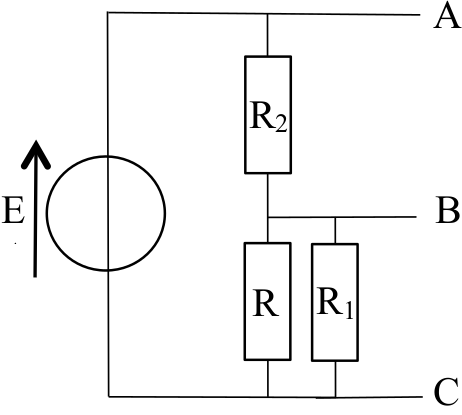
\includegraphics[height=3cm]{th_3_2.png}}
    \hspace{3cm}
    \subfloat[Schéma 2]{\label{fig:th2}
    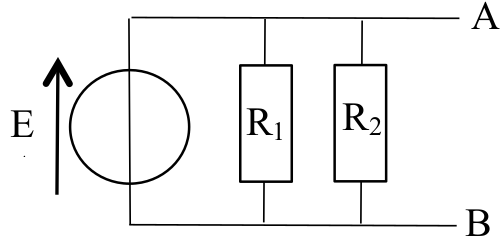
\includegraphics[width=4cm]{th_2_1.png}}
\end{figure}

Pour chacun des schémas ci-dessus, on veut déterminer les caractéristiques du
générateur de Thévenin équivalent entre les bornes A et B, sachant que $E =
\SI{15}{V}, R = \SI{10}{k\O}, R_1 = \SI{4.7}{k\O}, R_2 = \SI{1}{k\O}$. Pour cela
:

\begin{enumerate}[label=\color{brandeisblue}\arabic*)]
    \item Déterminez et calculez $E \St{th} = U \St{AB}$.
    \item Faites le schéma équivalent permettant de déterminer $R \St{th}$.
    \item Déterminez et calculez $R \St{th}$.
\end{enumerate}

\begin{minipage}[c]{0.49999\textwidth}
    \begin{center}
        Schéma 1
    \end{center}
    \raggedleft\vrule height 14cm
\end{minipage}%
\begin{minipage}[c]{0.49999\textwidth}
    \begin{center}
        Schéma 2
    \end{center}
    \vspace{14cm}
\end{minipage}

\newpage

\section{Générateur de Thévenin et puissance dissipée (14 points)}
\begin{wrapfigure}[5]{R}{.4\linewidth}
    \vspace*{-25pt}
    \raggedleft
    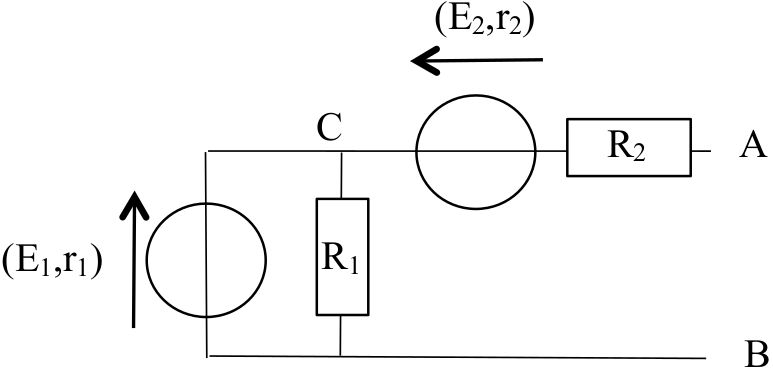
\includegraphics[width=\linewidth]{th_solo.png}
    \captionsetup{justification=centering}
    \caption{Schéma simplifié}
    \label{fig:solo}
\end{wrapfigure}
COnsidérons le circuit ci-contre, composé de 2 générateurs de tension \Ul{réels}
$(E_1, r_1)$ en parallèle avec $R_1$ et $(E_2, r_2)$ en série avec $R_2$. On
donne $E_1 = \SI{10}{V}, E_2 = \SI{5.0}{V}, r_1= \SI{5.0}{k\O}, r_2 =
\SI{1.0}{k\O}, R_1 = \SI{10}{k\O}, R_2 = \SI{20}{k\O}$.

\begin{enumerate}[label=\color{brandeisblue}\arabic*)]
    \item Redessiner le schéma complet normalisé en ne faisant apparaître que
        des générateurs idéaux de tension et des résistances.
        \vspace{3cm}
    \item Que peut-on dire du courant dans la branche $AC$ ?
        \vspace{1cm}
    \item Fléchez courants et tensions.
\end{enumerate}

\begin{enumerate}[label=\color{brandeisblue}\arabic*), resume]
    \item Déterminez l'expression littérale de $E \St{th} = U \St{AB}$ du
        générateur de Thévenin entre $A$ et $B$ et calculez sa valeur. Il faut 1
        additivité des tensions et 1 loi des mailles.
        \vspace{3cm}
    \item Faites le schéma équivalent permettant de déterminer $R \St{th}$,
        déterminez son expression littérale et calculez sa valeur.
        \vspace{3cm}
    \item Réprésentez le schéma équivalent avec le générateur de Thévenin,
        aux bornes duquel on a branché une résistance $R = \SI{25}{k\O}$.
        Déterminez l'intensité $I(R)$ la parcourant en fonction de $E \St{th}$
        et $R \St{th}$, et calculez sa valeur.
        \vspace{3cm}
    \item Exprimer la puissance $P(R)$ dissipée par la résistance en fonction de
        $E \St{th}, R \St{th}$ et $R$ et calculez sa valeur.
\end{enumerate}

\end{document}
